% !TeX spellcheck = en_GB
% \begin{figure}[h!]
% 	\centering
% 	\begin{subfigure}[b]{0.55\textwidth}
% 		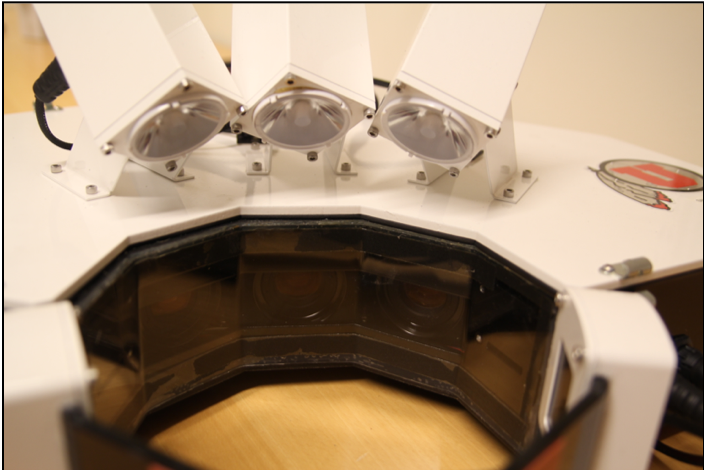
\includegraphics[width=\textwidth]{./fig_instruments/MASC.png}
% 	\end{subfigure}
% 	\begin{subfigure}[b]{0.55\textwidth}
% 		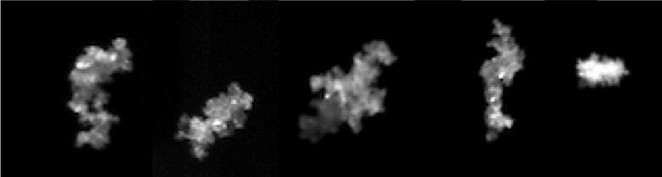
\includegraphics[width=\textwidth]{./fig_instruments/MASC_snowflakes.png}
% 	\end{subfigure}
% 	\caption{Instrument MASC, and images taken by the instrument. \textcolor{red}{lower panel taken from \cite{cooper_variational_2017} maybe we get one for Haukeli?}}\label{fig:MASC}
% \end{figure}

\begin{wrapfigure}[14]{r}{0.44\textwidth}
	\vspace{-\normalbaselineskip}
	\centering
	\begin{subfigure}[b]{0.4\textwidth}
		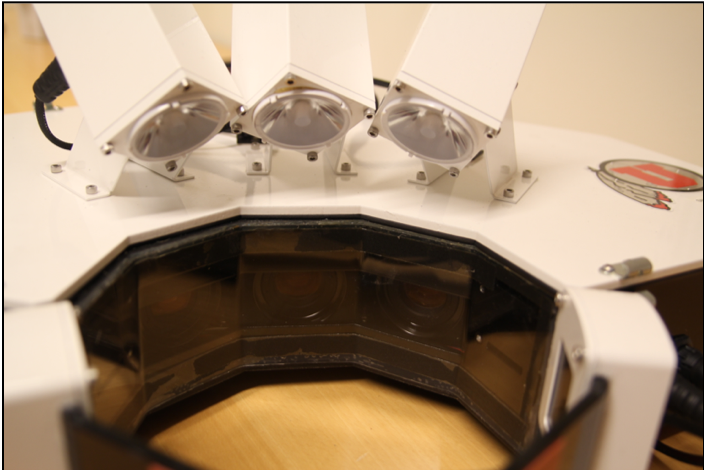
\includegraphics[width=\textwidth]{./fig_instruments/MASC.png}
	\end{subfigure}	
	\begin{subfigure}[b]{0.4\textwidth}
		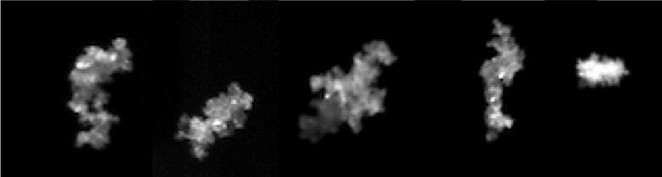
\includegraphics[width=\textwidth]{./fig_instruments/MASC_snowflakes.png}
	\end{subfigure}	
	\caption{MASC and images taken by instrument. \textcolor{red}{Lower panel taken from \cite{cooper_variational_2017} maybe we get one for Haukeli?}}\label{fig:MASC}
	%	\vspace{-\normalbaselineskip}
\end{wrapfigure}